\documentclass [11pt]{article}
\usepackage{filecontents}

\begin{filecontents}{data.txt}
age efrom elength ofrom olength
1994 6 6 12 2
1993 7 6 13 2
1992 6 6 12 4
1991 7 6 13 4
1990 4 8 12 4
1989 5 8 13 4
1988 6 6 12 4
1987 7 6 13 4
1986 8 4 12 4
1985 9 4 13 4
1984 10 2 12 4
1983 11 2 13 4
\end{filecontents}n

\usepackage[left = 0.4in, top = 0.33in, right = 0.4in, bottom = 0.6in]{geometry}
\usepackage[utf8]{inputenc}
\usepackage{array}
\usepackage[T1]{fontenc}
\usepackage{geometry}
\usepackage{tikz}
\usetikzlibrary{shapes.geometric, arrows}
\usetikzlibrary{shapes,positioning, intersections,quotes,fit}
\usepackage{pgfplots}
\usepackage{filecontents}
\usepackage{booktabs}
\usepackage{amsmath}
\usepackage{chronology}
\usepackage{float}
\usepackage{multicol}
\usepgfplotslibrary{fillbetween}
\usetikzlibrary{patterns}
\usepackage{multirow}
\usepackage{url}


\pgfplotsset{compat=1.12}
\usepackage{filecontents}
\begin{filecontents*}{data2.txt}
Year	under50	under50low	under50high	5064	5064low	5064high	
6	.15	0.1	0.2	0.1	0.05	0.15	
8	.2	0.12	0.24	0.12	0.05	0.17	
10	.05	-0.05	.12	0.02	-.1	.08
12	0	-0.1	0.1	0	-0.05		0.08		
\end{filecontents*}

\pgfplotsset{
	jitter/.style={
		x filter/.code={\pgfmathparse{\pgfmathresult+rnd*#1}}
	},
	jitter/.default=0.1
}


\title{Ph.D. Proposal Draft 3.2}
\author{Randall Boyes}
\date{August 14, 2018}
\begin{document}
\maketitle


\section{Introduction}
Outdoor active play is an important part of childhood development.~\cite{Curtis2012-ql,Pearce2008-lq,Pernsteiner2012-qm} Outdoor active play reduces sedentary behaviour, protects against obesity, and has an important role in the development of behaviours.~\cite{Ansari2015-ig} Children - both Canadian and international - indicate a strong desire for outdoor active play time, which is characterized by reduced rules and supervision, the ability to interact with other children, and variation in experiences.~\cite{Watson2016-qd,Caro2016-er,Herrington2015-pb} Canadian children have been engaging in fewer hours of outdoor active play over time. This decrease has been attributed to a number of societal changes, including increasing pressure on parents to protect their children from injury and from abduction, though the latter is quite rare.~\cite{Mitra2014-qg} While there are risks associated with outdoor active play in the short term which are a societal concern, children need physical activity. It is not clear what the risks of outdoor active play are as compared to other forms of physical activity such as organized sport. Further, outdoor active play contributes to child development and this reduction in play may have consequences for health and behaviour as they get older \cite{barker2014less}. 

According to the CDC, the behaviours that pose the greatest risk to adolescent health are substance use, including excessive alcohol use, tobacco use, and drug use; risky sexual behaviours; behaviours that result in injury; physical inactivity; and sedentary behaviour. Outdoor active play reduces sedentary behaviour and protects against obesity.~\cite{Ansari2015-ig} The lessons learned and skills obtained through outdoor active play may also be protective against these other health risk behaviours. By protecting children from injury and the perceived threat of abduction over the short term by limiting their exposure to unsupervised outdoor active play, parents could be exposing children to other long term risks, including chronic disease risk.

Both engagement in outdoor active play in children and health risk behaviour in adolescents are influenced by their physical and social environments.~\cite{Aarts2010-pk} Changes in this environment could be a contributing factor in the observed reduction in overall outdoor active play. Parks, green space, and low-traffic roads provide space to play in, and the social context of the neighbourhood influences both parents' willingness to allow children freedom and children's desire to be outside. But these environments could impact risk behaviour as well.~\cite{Wallace2017-kj,Spilkova2014-iv} Parks and other outdoor spaces that encourage outdoor active play in children could provide a place for adolescents to engage in risk behaviours. By considering the influence of the environment on both outdoor active play behaviours and risk behaviours, healthy behaviours can be encouraged in all age groups.

\subsection{Purpose}

This thesis will examine neighbourhood level determinants of outdoor active play and health risk behaviours, as well as relationship between outdoor active play and health risk behaviours at the individual level.  

\subsection{Objectives \& Hypotheses.} The goals of this thesis project are:
\begin{enumerate}
\item To investigate the association of a neighbourhood playability index with outdoor active play and health risk behaviour in children. I expect that higher neighbourhood playability will be associated with increases in both outdoor active play and health risk behaviour. 
\item To develop an understanding of the injuries that result from outdoor active play relative to the injuries that occur in other types of physical activity. I hypothesize that injuries from outdoor active play will be less severe and less frequent than organized sport injuries.
\item To determine the association of outdoor active play in childhood with adolescent risk taking behaviour. I predict that higher levels of outdoor active play in childhood will be associated with lower health risk behaviour in adolescence.
\end{enumerate}

\begin{figure}[h]
\centering
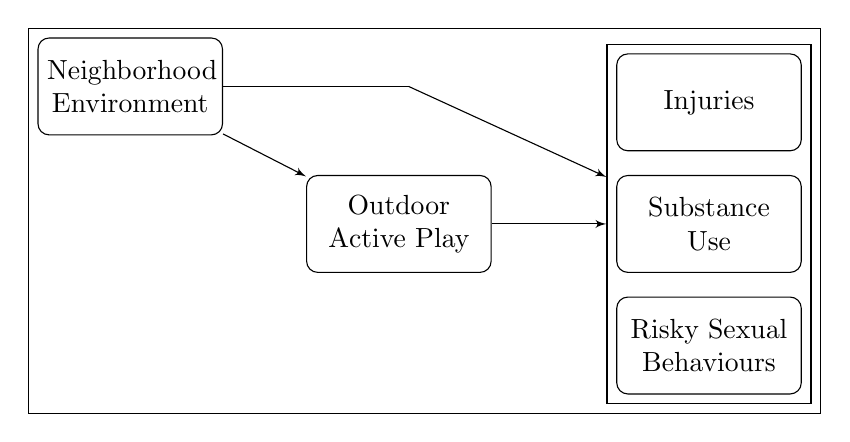
\begin{tikzpicture}[decision/.style={diamond, draw, text width=4.5em,text badly centered, node distance=3.5cm, inner sep=0pt},block/.style={rectangle, draw, text width=6em, text centered,rounded corners, minimum height=3.5em},cloud/.style ={draw, ellipse, minimum height=2em},line/.style ={draw,-latex'},node distance =1cm,auto]
\node [block] (1st1) {Neighborhood Environment};
\node [right = 6em of 1st1](c1){};
\node [block, below = 1 cm of c1] (2nd1)  {Outdoor Active Play};

\begin{scope}[node distance=3mm and 10mm]
\node [block, right= 45pt of 2nd1] (3rd1) {Substance Use};
\node [block, below = of 3rd1] (3rd0) {Risky Sexual Behaviours};
\node [block, above = of 3rd1] (3rd2) {Injuries};
\end{scope}

\node[draw,fit=(3rd0) (3rd2)] (box1){};

\node [below = 1em of box1.west](c2){};

\node[draw,solid,fit= (1st1) (box1)] (box2){};

\draw[line] (2nd1.east) -- (box1);
\draw[line] (1st1) -- (2nd1);
\path[draw] (1st1) -- (c1.east);
\path[line] (c1.east) -- (box1);

\end{tikzpicture}
\caption{Overall framework. Outdoor active play shapes health risk behaviour (injuries, substance use, risky sexual behaviours) at the individual level. Both outdoor active play and health behaviour are influenced by the neighbourhood environment.}
\label{m1fig}
\end{figure}












\section{Manuscript 1: Influence of the Built Environment}
\subsection{Introduction} 

Both physical and social environmental factors influence the behaviour of children and adolescents.~\cite{Glanz2015-of,Barker1968-vn,Moos1980-wh,Bronfenbrenner1977-hj,Glass2006-px,Moore2015-gr} Neighborhood social environment in particular has been shown to be one of the strongest predictors of outdoor active play; the social context of the neighbourhood influences both parents' willingness to allow children freedom and children's desire to be outside.~\cite{Remmers2014-ng} The physical environment is also associated with outdoor active play behaviour. Previous attempts to quantify the influence of the built environment on outdoor active play have mostly focused on specific contexts, such as playgrounds, but children engage in outdoor active play in a variety of settings, including - most commonly - near the home.~\cite{Aarts2012-dt} 

Increased traffic safety (as measured by the presence of sidewalks (OR 1.44 (1.16, 1.81) for boys, 1.66 (1.39, 1.99) for girls), speed, roundabouts (OR 1.15(1.06, 1.24)), and intersections (OR 0.81 (0.73, 0.90)) in the neighborhood are positively correlated with outdoor active play.~\cite{Aarts2010-pk,Aarts2012-dt} Additional neighbourhood characteristics have been shown to be associated with children's physical activity and could relate to rates of outdoor active play as well, including Walkability, number of parks and playgrounds, tight social networks, positive peer influence, and neighborhood safety, recreation facilities, traffic density, walking and cycling infrastructure, both crime-related and subjective safety, and neighborhood aesthetics \cite{Timperio2015-wn}. +

Neighborhood features have the potential to directly influence health risk behaviours as well.. Hillier hypothesized that there are two classes of space users: `ordinary citizens', who use space to go about their everyday business; and `space explorers', whose goals are to explore the potential of space.~\cite{Wallace2017-kj,Spilkova2014-iv,noauthor_undated-pd} Children looking for places to play and adolescents looking for places to engage in substance use can both be considered `space explorers' in Hillier's framework. Therefore, it may be that the very parks and other outdoor spaces that encourage outdoor active play in children could provide a place for adolescents to engage in health risk behaviours. 

\subsection{Purpose}

This initial study will measure the impact of neighbourhood-level features of the built environment as measured by a playability index on both outdoor active play and health risk behaviours. 

\begin{figure}
\centering
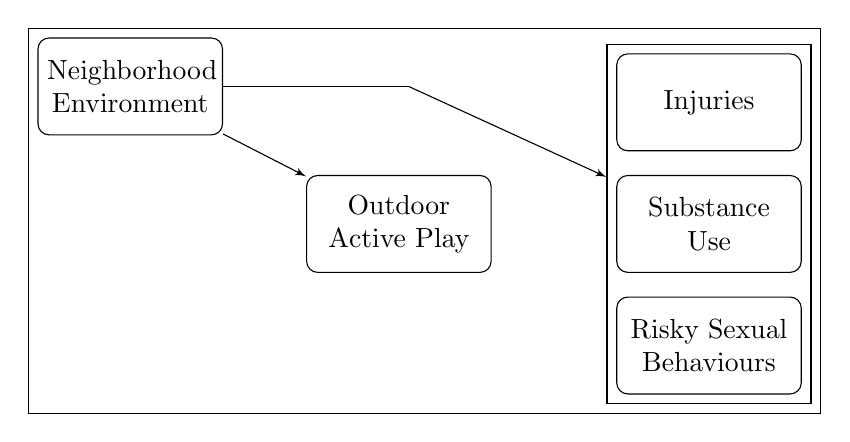
\begin{tikzpicture}[decision/.style={diamond, draw, text width=4.5em,text badly centered, node distance=3.5cm, inner sep=0pt},block/.style={rectangle, draw, text width=6em, text centered,rounded corners, minimum height=3.5em},cloud/.style ={draw, ellipse, minimum height=2em},line/.style ={draw,-latex'},node distance =1cm,auto]
\node [block] (1st1) {Neighborhood Environment};
\node [right = 6em of 1st1](c1){};
\node [block, below = 1 cm of c1] (2nd1)  {Outdoor Active Play};

\begin{scope}[node distance=3mm and 10mm]
\node [block, right= 45pt of 2nd1] (3rd1) {Substance Use};
\node [block, below = of 3rd1] (3rd0) {Risky Sexual Behaviours};
\node [block, above = of 3rd1] (3rd2) {Injuries};
\end{scope}

\node[draw,fit=(3rd0) (3rd2)] (box1){};

\node [below = 1em of box1.west](c2){};

\node[draw,solid,fit= (1st1) (box1)] (box2){};

\draw[line] (1st1) -- (2nd1);
\path[draw] (1st1) -- (c1.east);
\path[line] (c1.east) -- (box1);

\end{tikzpicture}
\caption{Manuscript one framework. Both outdoor active play and health risk behaviours (injuries, substance use, risky sexual behaviours) are associated with differences in the neighbourhood environment.}
\label{basicfig}
\end{figure}



\subsection{Objectives} 

\begin{enumerate}
\item To validate an index of playability that incorporates the features of the built environment of a child's neighbourhood which are associated with outdoor active play.
\item To determine the association between this playability index and outdoor active play and health risk behaviours after controlling for individual-level confounding variables.  
\end{enumerate}

\subsection{Study Design and Data Source} 

\paragraph{Study Design. }This is a cross sectional study. 

\paragraph{Data Source.} The data source is the 2014 cycle of the Health Behaviour in School-aged Children Survey. The 2014 HBSC involved a national survey of 29,784 students from 377 schools from across Canada. A subset of this study (subject to inclusion criteria below) will form the study population.  

\paragraph{Inclusion and Exclusion.} Inclusions:  (1) Participated in the 2014 HBSC; (2) grades 6 to 8 (ages 11-13); (3) attended a school in a public or separate board; (4) reported a valid postal code for their residential address.  16,290 young people met these inclusion criteria.

\subsection{Measurement} 

\paragraph{Exposure: Playability.} A neighbourhood playability index, which is being developed by the Playability Project team at UBC, a CIHR-funded interdisciplinary group of researchers led by Mariana Brussoni and Louise Masse, will be tested using the HBSC data. It will include features of neighbourhoods such as number of parks, amount of green space, presence of traffic safety features, and neighbourhood road connectivity. The goal of this index is to define features of neighbourhoods that predict childrens' engagement in outdoor active play. The neighbourhood of a child will be determined using a set distance (1 km) by road from the midpoint of the area represented by their reported home postal code. I will measure the aspects of the playability index that are available in the HBSC data which predict outdoor active play. These features will be measured by primary data collection via geographic information systems analysis, as per precedents in the Janssen laboratory.~\cite{Carson2014-xh} 

\paragraph{Outcome 1: Outdoor Active Play.} The number of hours of outdoor active play are assessed on the HBSC using the questions: `On weekdays, how many hours a day do you usually spend time playing outdoors outside school hours?' and `On weekends, how many hours a day do you usually spend time playing outdoors outside school hours?' The possible responses to each of these questions were: `none at all', `half an hour', `1h', `2h', `3h', `4h', `5h', `6h', and `7h or more.' A total number of hours per week spent in outdoor active play will be estimated from these questions. 

\paragraph{Outcome 2: Health Risk Behaviour.} The HBSC includes questions on frequency of health risk behaviours, including frequency of binge drinking (5 or more drinks in one day), cigarette smoking, smokeless tobacco use, cannabis use, injuries, and risky sexual behaviours. Tests of self reported measures like the ones used here for substance use versus urinalysis show sensitivity and specificity of approximately 80\%.~\cite{Akinci2001-nd,Murphy2000-fy,Brener2003-ps} Self reported smoking measures have even higher sensitivities and specificities of approximately 90\%.~\cite{Post2005-yw} These measures of these behaviours have previously been combined to form a single continuous score.~\cite{Kwong2017-oe} 

\paragraph{Confounders and Effect Modifiers:} Sex, age, certain disabilities, rurality, ethnicity, self-reported SES, sleep, family structure, and family attachment can be measured using the HBSC. See Section 5 for evidence of relationships and below for selection process. 

\subsection{Statistical Analysis:} 

\subsubsection{Objective 1: Validation of the Playability Index.}

Qualitative results from the Playability project will be tested using HBSC data. The purpose of the Playability Index is to correlate with the rate of outdoor active play for any given neighbourhood. In order to avoid overfitting, model fit will be checked in bootstrapped samples. Different modelling strategies will be tested to find the best strategy. Models will differ by variable inclusion and functional form of the included variables.  As we are aiming to generate a continuous score with an interpretable model, possible models include penalized GLMs such as lasso or ridge regression.   

\subsubsection{Objective 2: Associations with the Playability Index.}

\paragraph{Assumptions for Causal Inference:} Making causal inferences about neighbourhood factors in this context is difficult; in fact, arguments have been made that suggest that causal inference in this context cannot be done.~\cite{Oakes2004-jw} Such arguments rest on (amoung other things) violations of the exchangeability and positivity assumptions - that is, it is believed that ''a similar person in a different neighbourhood'' does not exist due to self-selection of participants into neighbourhoods. Causal inference may still be possible due to the population of interest being children, who typically do not choose their neighbourhood.

\paragraph{Modelling Strategy:} As the HBSC is uses a clustered sampling approach, the models of the associations between neighbourhood playability and outdoor active play and health risk behaviours will need to be mixed effects models. Random effects for neighbourhood, school, and class will be used to correct the estimates of variance. Effect estimates will be relative risks for binary outcomes (using log-binomial mixed effects models) or slopes for continuous outcomes. 

\paragraph{Power:} Assuming a sample size of 16,290 spread over 377 clusters with estimate of 0.10 for the intraclass correlation coefficient based on previously calculated intraclass correlation coefficients for binge drinking and smoking in this data set for 15 year olds \cite{BOYES2017663}, the design effect can be calculated as:

\begin{equation}\nonumber
D = 1 + \rho (k - 1)
\end{equation}
\begin{equation}\nonumber
D = 1 + 0.10 (16290/377 - 1)
\end{equation}
\begin{equation}\nonumber
D = 5.22
\end{equation}

If a simple comparison was done between high playability and low playability neighborhoods, the minimum detectable effect would be 0.91 standard deviations at 80\% power, 1.06 standard deviations at 90\% power, or 1.17 standard deviations at 95\% power.~\cite{Galecki2009-jt} For categorical variables, 80\% power is attained at a true relative risk of approximately 1.35. 

\paragraph{Covariates.}

In order to estimate the relationship between neighborhood factors and outdoor active play behaviour, the models will need to control for both neighborhood- and individual-level confounding variables. Confounder selection can be based on the minimal subset of variables that close all back door paths from exposure to outcome as long as an accurate DAG can be drawn. \cite{VanderWeele2011-xu} Plausible causes of the built environment in which children grow up include physical health, socioeconomic status, ethnicity, and family structure, attachment, and environment. These variables could be causally related to neighbourhood built environment by influencing the parent's choice of where to live. Variables such as sleep duration, sex, and age, which are not causes of built environment factors, will not be controlled for. Effect modification by sex and age will be investigated. More detail and some additional potential covariates are listed in Section 5: Potential Covariates. 

\paragraph{Sensitivity Analysis by Rurality.}

Because exposure information is being collected by postal code, assessment of the neighbourhood where a child lives will be more accurate in urban areas than in rural areas. A sensitivity analysis will be conducted where the sample is restricted to non-rural areas, as defined by Statistics Canada. \cite{Government_of_Canada_Statistics_Canada2011-ee}

\section{Manuscript 2: Outdoor Active Play and Injury}
\subsection{Background and Rationale}

Caregivers limit childrens' freedom to participate in outdoor active play because they perceive this behaviour as being unacceptably dangerous, though the degree of concern depends on child-level factors including age, competence, and gender.~\cite{Mitra2014-qg, Lee2015-nz}  However, there is a lack of basic descriptive data on injuries that occur during outdoor active play. By quantifying this risk and comparing it to other common activities, we can enable decision making at both the social and parental level. 

Rates of injury in the context of the playground has been studied extensively, but there is little agreement between studies. A systematic review of play injuries in child care centres found injury rate estimates varied from 0.006 to 8.29 injuries per child-year, depending on the definition of ''injury.'' \cite{Hashikawa2015-nc} Outdoor injuries in general in children have been shown to result from play, sport, and transport, with trampolines, bicycles, and skis being frequent causes.~\cite{Gyllencreutz2015-ng,Klimek2013-er,Eager2013-dt} 

\subsection{Purpose}

This study aims to describe outdoor active play injuries and to compare the patterns of injury in outdoor active play with those experienced during alternative forms of physical activity. 

\begin{figure}[h]
\centering
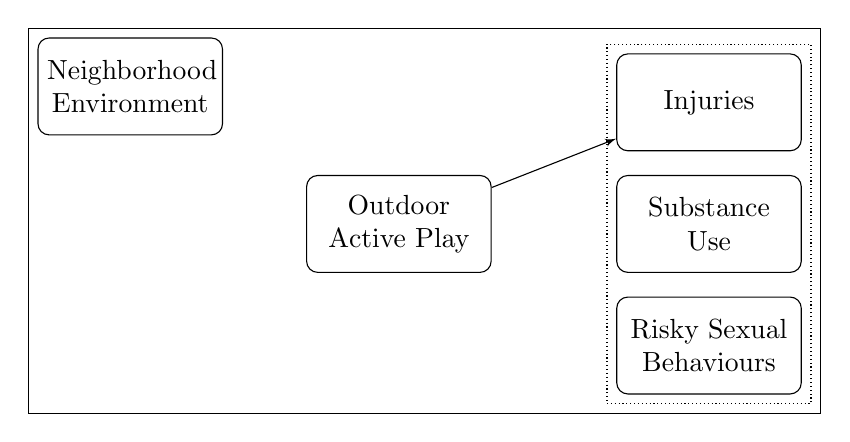
\begin{tikzpicture}[decision/.style={diamond, draw, text width=4.5em,text badly centered, node distance=3.5cm, inner sep=0pt},block/.style={rectangle, draw, text width=6em, text centered,rounded corners, minimum height=3.5em},cloud/.style ={draw, ellipse, minimum height=2em},line/.style ={draw,-latex'},node distance =1cm,auto]
\node [block] (1st1) {Neighborhood Environment};
\node [right = 6em of 1st1](c1){};
\node [block, below = 1 cm of c1] (2nd1)  {Outdoor Active Play};

\begin{scope}[node distance=3mm and 10mm]
\node [block, right= 45pt of 2nd1] (3rd1) {Substance Use};
\node [block, below = of 3rd1] (3rd0) {Risky Sexual Behaviours};
\node [block, above = of 3rd1] (3rd2) {Injuries};
\end{scope}

\node[draw,densely dotted,fit=(3rd0) (3rd2)] (box1){};

\node [below = 1em of box1.west](c2){};

\node[draw,solid,fit= (1st1) (box1)] (box2){};

\draw[line] (2nd1) -- (3rd2);

\end{tikzpicture}
\caption{Manuscript two framework. Outdoor active play can lead to directly to injuries in the short term.}
\label{m2fig}
\end{figure}


\subsection{Research Question(s)} What types of injuries occur when children engage in outdoor active play? Are these injuries different in severity, frequency, anatomical site, or nature from the injuries that occur when children engage in more structured activities (i.e., active transport, school-based organized activities, or organized sports)? 

\subsection{Study Design} Descriptive. 

\subsection{Inclusion and Exclusion.} Children aged 5 to 14 who presented to hospital with an injury resulting from physical activity in Kingston between 2008 and 2018. This age range was chosen for developmental relevance and to align with census age categories. \cite{truelove2017defining, Government_of_Canada2017-iu}. 

\subsection{Data Source} 

Data describing injuries that presented for medical care in Kingston and the surrounding area will be obtained from the Canadian Hospital Injury Reporting and Prevention Program (CHIRPP) database, which captures injuries in patients reporting to emergency departments of the Kingston Health Sciences Centres (formerly Hotel Dieu and Kingston General Hospital). CHIRPP includes information on: 1. What was the injured person doing when the injury occurred? 2. What went wrong? 3. Where did the injury occur? and 4. The nature and anatomical site of the injury. 

\paragraph{Injury Rates.} In order to calculate rates, both the numerator (the number of injuries resulting from each type of physical activity) and the denominator (the number of children of each age and sex who were at risk) need to be measured. 

\paragraph{Number of Injuries.} Injuries that result from physical activity, including outdoor active play, will be identified based on open and close-ended codes describing where the injury occurred and what the child was doing, as well as narrative case descriptions. Participants are asked to indicate whether the injury in question happened indoors or outdoors and to indicate the specific activity they were participating in from a list which includes ''playing'' as an option. We expect that approximately 80\% of outdoor active play-related injuries will be identified using these questions, however, cases will exist that are coded as ''unknown.'' For these cases, identification will be attempted using the narrative entry (Section 5). Automated methods exist for topic detection in this type of narrative, such as Latent Dirichlet Allocation\cite{Blei2003-ob}, and will be used if necessary. Latent Dirichlet Allocation has been used in the past to extract topics from patient narratives \cite{Hassanali2013-va,Cohen2014-fd} Simpler methods involving keywords can also be used.~\cite{Fridman2013-wq} All cases will be classified based on the description of where the injury took place, what the child was doing, and who they were with, as available. The injury classification system will need to be developed as part of this thesis project, which represents a substantial time commitment.

\paragraph{Number of Children at Risk.} This study will focus on data from the Kingston Health Sciences Centre.~\cite{Pickett2003-zj} The catchment area of these two hospitals is approximated by the census population of the city of Kingston, Frontenac county, and Lennox \& Addington county.~\cite{Pickett2003-zj} Population by age and geographic region cross-tabulations are publicly available for the regions in question from the 2006, 2011, and 2016 censuses.~\cite{Government_of_Canada2007-zb,Government_of_Canada2017-iu} Populations at the years between censuses can be approximated via linear interpolation. This allows the number of person-years at risk in each age/sex strata to be determined. Unfortunately, we cannot determine risk per hour of activity, which means that comparisons will be done with cumulative incidence rates rather than rates per person-hour. 

\subsection{Presentation and Comparisons of Interest.} 

\paragraph{Estimates.} Injuries will be described according to nature and anatomical site of injury; activity leading to injury; location where the injury occured; and severity of injury. Descriptive tables will be created to show frequency of injury by category of physical activity. Patterns by age, sex, and location (if available) will also be reported. Illustration of typical or recurrent patterns of injury with vignettes will be explored as appropriate.~\cite{Pickett2003-zj}

\paragraph{Precision.} If there are 2000 injuries per year, split evenly between injuries in outdoor active play, sport, active transport, and school based activity, and between sexes, then we would observe 250 events in each sex/type stratum per 16,285 person years (2016 Kingston population ages 5 - 14). This would correspond to a incidence rate estimate of 1.54 (1.35, 1.73) per 100 children per year (poisson confidence interval). The rates of injuries are not expected to all be equal. If there is a category with half the expected rate, its rate estimate would be 0.76 (0.63, 0.90) per 100 children per year. 


\section{Manuscript 3: Outdoor Active Play and Future Health Behaviour}

\subsection{Rationale} 

Outdoor active play is an important part of children's development. Outdoor active play helps to form ideas, teach skills, and shape behaviour; some of which may carry forward into adolescence. Outdoor active play may have different effects on behaviour at different ages. Studies in neuroplasticity suggest that the brain is most susceptible to changes when we are young.~\cite{Mundkur2005-ws} 

According to the CDC, there are six main categories of behaviour that endanger health in adolescence: 1. Behaviours that contribute to unintentional injury and violence, 2. sexual behaviours that lead to unwanted pregnancies and STIs, 3. use of alcohol and other drugs, 4. tobacco use, 5. unhealthy dietary behaviours, and 6. inadequate physical activity.  The first four of these behaviours have been observed to cluster together, suggesting that there may be common underlying causes for all of them.~\cite{Kwong2017-oe,Noble2015-yd} 

Problem Behavior Theory \cite{Jessor1987-wz} suggests that different overt risk taking behaviours (substance use, violence, and risky sexual behavior) are motivated by similar personality characteristics and social influences.~\cite{Mobley2013-ij} This theory is supported by the fact that these overt risk behaviours have been shown to correlate with each other in the HBSC.~\cite{Kwong2017-oe} While it is not known for certain which specific personality characteristics account for this connection, there are some candidate characteristics that are also influenced by outdoor active play. These factors include incorrect evaluations of risk~\cite{Couch2017-tb}, an external locus of control, decreased executive function, an inability to connect with peers in a healthy way, and poor strategies for coping with stress.~\cite{Unger2016-qm,Johnson2002-qf,barker2014less} 

\subsection{Purpose}

This study will longitudinally examine the effect of childhood play on adolescent risk taking behaviours. 




	\begin{figure}[h]
	\centering
	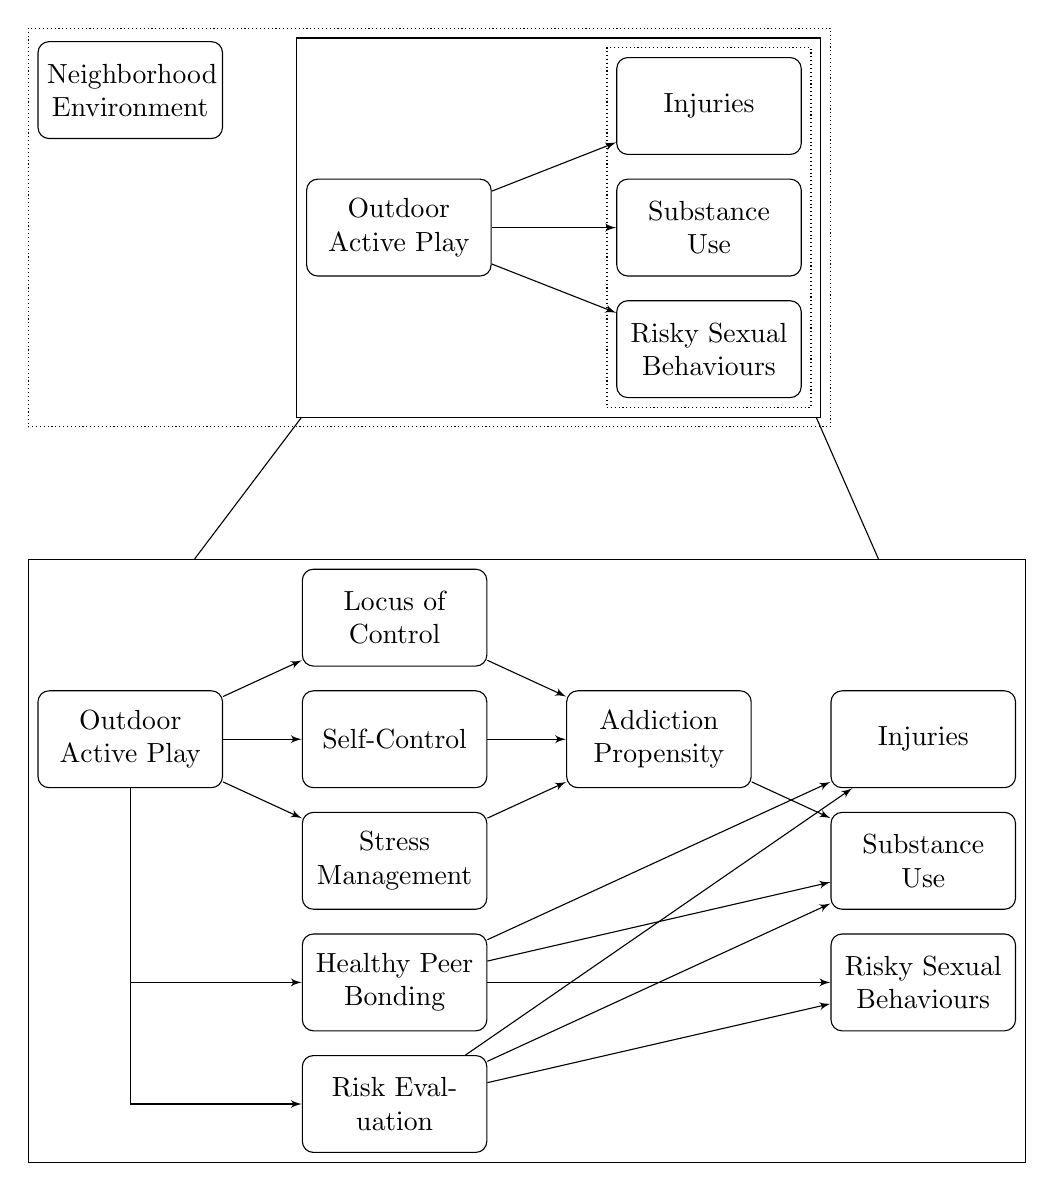
\begin{tikzpicture}[decision/.style={diamond, draw, text width=4.5em,text badly centered, node distance=3.5cm, inner 	sep=0pt},block/.style={rectangle, draw, text width=6em, text centered,rounded corners, minimum 					height=3.5em},cloud/.style ={draw, ellipse, minimum height=2em},line/.style ={draw,-latex'},node distance =1cm,auto]
		\node [block] (1st1a) {Neighborhood Environment};
		\node [right = 6em of 1st1a](c1){};
		\node [block, below = 1 cm of c1] (2nd1a)  {Outdoor Active Play};

		\begin{scope}[node distance=3mm and 10mm]
		\node [block, right= 45pt of 2nd1a] (3rd1a) {Substance Use};
		\node [block, below = of 3rd1a] (3rd0a) {Risky Sexual Behaviours};
		\node [block, above = of 3rd1a] (3rd2a) {Injuries};
		\end{scope}
	
		\node[draw,densely dotted,fit=(3rd0a) (3rd2a)] (box1){};
	
		\node [below = 1em of box1.west](c2){};

		\node[draw,solid,fit= (2nd1a) (box1)] (box4){};
		\node[draw,densely dotted,fit= (1st1a) (box4)] (box2){};


		\draw[line] (2nd1a) -- (3rd2a);
		\draw[line] (2nd1a) -- (3rd1a);
		\draw[line] (2nd1a) -- (3rd0a);
\node [block, below = 7 cm of 1st1a] (1st) {Outdoor Active Play};
\node [block, right= of 1st] (2nd1) {Self-Control};

\begin{scope}[node distance = 25mm]
\end{scope}

\begin{scope}[node distance=3mm and 10mm]
\node [block, above= of 2nd1] (2nd2) {Locus of Control};
\node [block, below= of 2nd1] (2nd3) {Stress Management};
\node [block, right= of 2nd1] (3rd1) {Addiction Propensity};
\node [block, below = of 2nd3] (2nd4) {Healthy Peer Bonding};
\node [block, below = of 2nd4] (2nd5) {Risk Evaluation};
\node [block, right= of 3rd1] (4th1) {Injuries};
\node [block, below = of 4th1] (4th0) {Substance Use};
\node [block, below = of 4th0] (4th2) {Risky Sexual Behaviours};
\end{scope}

\path [line] (1st) -- (2nd1);
\path [line] (1st) -- (2nd2);
\path [line] (1st) -- (2nd3);
\path [line] (2nd1) -- (3rd1);
\path [line] (2nd2) -- (3rd1);
\path [line] (2nd3) -- (3rd1);
\path [line] (3rd1) -- (4th0);
\path [line] (1st) |- (2nd4);
\path [line] (1st) |- (2nd5);
\path [line] (2nd5) -- (4th2);
\path [line] (2nd5) -- (4th1);
\path [line] (2nd5) -- (4th0);
\path [line] (2nd4) -- (4th0);
\path [line] (2nd4) -- (4th2);
\path [line] (2nd4) -- (4th1);

\node[draw,solid,fit=(1st) (2nd2) (4th0) (2nd5)] (box3){};

\node [right = 8.6em of box4.south](c6){};
\node [left = 8.6em of box4.south](c7){};
\node [right = 12em of box3.north](c8){};
\node [left = 12em of box3.north](c9){};

\path[draw] (c6.east) -- (c8.east);
\path[draw] (c7.west) -- (c9.east);



\end{tikzpicture}
\caption{Potential mechanisms behind of the relationship between outdoor active play in childhood and risk taking behavior in adolescence. Outdoor active play could influence childrens' locus of control, self-control, stress management and/or peer bonding strategies, or evaluation of risk. These traits influence attitudes towards health risk behaviours.}
\label{overall}
\end{figure}




\subsection{Research Question(s)} 
\begin{enumerate}
\item Is outdoor active play in childhood influence associated with health risk behaviours in adolescence? If so, at what age is this association strongest? 
\item Has this association between outdoor active play and health risk behaviours changed over time? 
\end{enumerate}

\subsection{Study Design} Secondary Analysis of a Prospective Cohort Study. 

\subsection{Data Source} This study will be a secondary analysis of data from the National Longitudinal Survey of Children and Youth (NLSCY), a 14 year longitudinal study of young Canadians. Cycle 1 data were collected in 1994 and consisted of 16,903 children aged 0 - 11 years. This group was surveyed again every two years until 2008 (remaining n = 10,268). This is the most recent longitudinal Canadian data source for this age group that includes the questions needed, but children today may not be the same as the children who participated in this study. 

\subsection{Inclusion and Exclusions} All children who responded to the original survey and remained in the cohort for at least one outcome observation will be included in this study. The population of the original survey includes non-institutionalized civilians residing in one of the ten Canadian provinces. The survey excludes children living on First Nations reserves or Crown lands, residents of institutions, children of full-time members of the Canadian Armed Forces, and residents of some remote regions.~\cite{Government_of_Canada2009-ep}

\subsection{Measurement}
\paragraph{Exposure: Outdoor Active Play.} If the children were between 4 and 9 years of age, their PMK (Person most knowledgeable) was asked: `In the last 12 months, outside of school hours, how often has [child's name] taken part in unorganized sports or physical activities?' This was changed to `...taken part in unorganized sports or physical activities \emph{without a coach or instructor}?' and the age was modified to only include 6 to 9 year olds in Cycle 2. In Cycle 4, the minimum age was reduced to 3, where it remained until the final Cycle in 2008. Additionally, children aged 10 and older were asked to indicate how often: `Outside of school, I play sports or do physical activities WITHOUT a coach or instructor.' The wording was updated in Cycle 2 to include `(biking, skateboarding, etc.)' Children ages 14 and older are not asked about play outside of school. The typical child in the dataset will have their frequency of outdoor active play measured at 4 time points with 2 years between measurements (See Figure 5 for example). 

\paragraph{Outcome: Health Risk Behaviour.} For cycles completed between the ages of 13 and 17, the participants filled out a questionnaire that asked questions about health risk behaviour including substance misuse, failure to take health precautions, and engagement in activities that place the child at physical or emotional risk (e.g. illegal activities). The questions on substance use behaviour come from the Youth Smoking Survey, the HBSC, the Northwest Territories Health Attitudes, Knowledge, and Behaviours Study, the Western Australia Child Health Survey, and the National Longitudinal Survey of Youth at Ohio State University. Tests of self reported measures of substance use like the ones used here versus urinalysis show sensitivity and specificity of approximately 80\%.~\cite{Akinci2001-nd,Murphy2000-fy,Brener2003-ps} An overall health risk behaviour score similar to the one derived from the HBSC questions in Manuscript 1 will be derived from response patterns on these questions.~\cite{Pickett2006-jz,Koven2005-mj} 

\paragraph{Potential Covariates:} See Section 5 for potential confounders and effect modifiers. These measurements are based on self-reported data from the NLSCY questionnaire. 

\begin{figure}
\centering
\begin{chronology}[2]{1994}{2009}{10cm}
\event[\decimaldate{01}{01}{1996}]{\decimaldate{31}{12}{1996}}{$X_0$}
\event[\decimaldate{01}{01}{1998}]{\decimaldate{31}{12}{1998}}{$X_1$}
\event[\decimaldate{01}{01}{2000}]{\decimaldate{31}{12}{2000}}{$X_2$}
\event[\decimaldate{01}{01}{2002}]{\decimaldate{31}{12}{2002}}{$X_3$ and $Y_3$}
\event[\decimaldate{01}{01}{2004}]{\decimaldate{31}{12}{2004}}{$Y_4$}
\event[\decimaldate{01}{01}{2006}]{\decimaldate{31}{12}{2006}}{$Y_5$}
\end{chronology}

\begin{tabular}{p{.85cm} m{.8cm} m{.8cm} m{.8cm} m{.8cm} m{.8cm} m{.8cm} m{1cm}}
\toprule
Age & 6 & 8 & 10 & 12 & 14 & 16 & \\
Time & $t_0$ & $t_1$ & $t_2$ & $t_3$ & $t_4$ & $t_5$ & \\
Cycle & 2 & 3 & 4 & 5 & 6 & 7 \\
\end{tabular}
\caption{Exposure and outcome measurement for a single example individual.}
\end{figure} 


\subsection{Statistical Analysis} Care will be taken to ensure that the results obtained from models are interpretable. High priority will be placed on clear explanations of findings through figures and simple tables. Confounder selection will be based on an attempt to select the smallest subset of variables that is sufficient to close all backdoor paths from exposure to outcome. The effects of misclassification and missing data will be considered. 

\subsubsection{Objective 1: Is play related to Health Risk Behaviour?}

Sequential conditional mean models \cite{Keogh2018-ra} will be used to estimate the total effect of outdoor active play on health risk behaviours. A separate model will need to be fit for each combination of outdoor active play at each measured time point (X\textsubscript{0} to X\textsubscript{3}) and the outcome at each time point (Y\textsubscript{3} to Y\textsubscript{5}), controlling for confounders at the same time as the exposure of interest (L\textsubscript{0} to L\textsubscript{3}). This approach relies on the assumption that outdoor active play after t\textsubscript{3} either does not occur or has no effect on the outcome. Generalized estimating equations can be used to estimate the coefficients, but prior exposure and outcome history need to be controlled for to obtain unbiased estimates.~\cite{Keogh2018-ra} The models are then of the general form:

\begin{equation}\nonumber
E(Y_t|X_{t-a}, L_{t-a}) = \beta_0  + \beta_{X_2} X_{t-a}  + \beta_{X_1} X_{t-a-1} + \beta_Y Y_{t-1} + \beta_{L_{t-a}}^T L_{t-a}
\end{equation}

For t = (3, 4, 5) and a = (1, 2, 3, 4), except for the combination t = 3 and a = 4. These 11 models represent the total effect of outdoor active play at each time point on health risk behaviours at each time point. In addition, if a propensity score can be estimated which balances covariates, then the models will control for this score as well. A propensity score would need to model the likelihood of engaging in outdoor active play, and would include variables such as age, sex, ethnicity, and SES. Controlling for propensity score gives doubly robust estimators of the exposure effect and down-weights exposed individuals who have no comparable unexposed counterparts.~\cite{Keogh2018-ra} Estimates of effect could be presented in a figure similar to Figure 6. 

\begin{figure}[H]
\centering
\begin{tikzpicture}
\begin{axis}[jitter,
ytick={-0.20,-0.15,...,0.30},
yticklabels = {-0.20,-0.15,-0.10,-0.05,0,0.05,0.10,0.15,0.20,0.25,0.30},
xtick={6,8,10,12},
ymax = 0.30,
xmin = 5, xmax = 13,
legend pos = north east,
xlabel = Age, ylabel = Estimated Effect,
height = 7cm
]
\node[] at (axis cs: 6.5,0.25) {Age 14};
\addplot+ [
error bars/.cd,
y explicit,
y dir=both,
] table [
x=Year,
y=under50,
y error plus expr=\thisrow{under50high} - \thisrow{under50},
y error minus expr=\thisrow{under50} - \thisrow{under50low},
] {data2.txt};
\addplot+ [
error bars/.cd,
y explicit,
y dir=both,
] table [
x=Year,
y=5064,
y error plus expr=\thisrow{5064high} - \thisrow{5064},
y error minus expr=\thisrow{5064} - \thisrow{5064low},
] {data2.txt};
\addplot [mark=none, densely dotted, domain = 5:13] {0};

\addlegendentry{Boys}
\addlegendentry{Girls}
\end{axis}


\end{tikzpicture}
\caption{Example plot of associations between exposure at all times and outcome at a specific time point, stratified by sex.}
\end{figure}

\subsubsection{Objective 2: Age, Period, and Cohort Effects}
There are three potential concurrent temporal effects in the data. 1. The age of the child is increasing. Differences in effect by age are what we wish to measure. 2. The year of measurement varies. If changes in the built and social environment external to the child interact with the effect of outdoor active play, then we would expect the year of measurement to be important. Such changes can affect all measurements taken in a given year, regardless of age. This type of effect is referred to as a `period' effect. 3. People born in different years may be fundamentally different. This is a `cohort' effect. These three effects suffer from the `identification problem.' That is, fundamentally:

\begin{equation}
\mbox{Age} = \mbox{Period} - \mbox{Cohort} \nonumber
\end{equation}

And so there is logically no statistical procedure that can separate their effects without further assumptions being made. Graphically, this can be seen in Figure 7: `Ten year olds who were measured in Cycle 1' and `Ten year olds who were born in 1984' are equivalent groups. One potential assumption that can be used is to assume that long term period effects have no trend, which effectively assumes that any trends that do show up in the data are cohort effects.~\cite{Bell2016-el} This assumption is not without costs; intervention strategies differ based on whether temporal trends are assumed to be cohort effects (the only effective interventions occur early in life) or period effects (interventions could be effective at any point). Given this assumption, the analysis described for objective 1 can be repeated in subgroups by birth year to examine changes over time. Any changes would be interpreted as cohort effects.  



\begin{figure}[h]
\centering
\begin{tikzpicture}
\begin{axis}[ytick=data, yticklabels from table={data.txt}{age}, grid=both,
width=15cm, height=10cm, axis background/.style={fill=white},
major grid style={gray!10}, xtick={0,...,17}, tick style={draw=none},
separate axis lines, axis line style={draw opacity=0}, xlabel ={Age}, ylabel={Year of Birth}]
% Lines
\addplot [blue, only marks, mark=*, error bars/.cd, error mark=none, x dir=both, x explicit]
table [x=efrom, y expr=\coordindex, x error plus=elength] {data.txt};
\addplot [red!70, only marks, mark=*, error bars/.cd, error mark=oplus*, x dir=both, x explicit]
table [x=ofrom, y expr=\coordindex, x error plus=olength] {data.txt};
	\draw [thin, dashed] (3,3) -- (12,12);
	\draw [thin, dashed] (3,1) -- (14,12);
	\draw [thin, dashed] (4,0) -- (16,12);
	\draw [thin, dashed] (6,0) -- (17,11);
	\draw [thin, dashed] (8,0) -- (17,9);
	\draw [thin, dashed] (10,0) -- (17,7);
	\draw [thin, dashed] (12,0) -- (17,5);
	\draw [thin, dashed] (14,0) -- (17,3);
	\draw [thick] (3,-1) -- (3,13);
	\node [below = 1pt of {(11,12)}, outer sep=2pt,fill = white] {1};
	\node [below = 1pt of {(13,12)}, outer sep=2pt,fill = white] {2};
	\node [below = 1pt of {(15,12)}, outer sep=2pt,fill = white] {3};
	\node [below = 2pt of {(17,11)}, outer sep=2pt,fill = white] {4};
	\node [below = 2pt of {(17,9)}, outer sep=2pt,fill = white] {5};
	\node [below = 2pt of {(17,7)}, outer sep=2pt,fill = white] {6};
	\node [below = 2pt of {(17,5)}, outer sep=2pt,fill = white] {7};
	\node [below = 2pt of {(17,3)}, outer sep=2pt,fill = white] {8};
	\node [right = 20pt of {(3,10)}, outer sep=2pt,fill = white] {Prior to 1994};
	\node [right = 28pt of {(3,9)}, outer sep=2pt,fill = white] {(No Data)};
\end{axis}
\end{tikzpicture}
\begin{center}
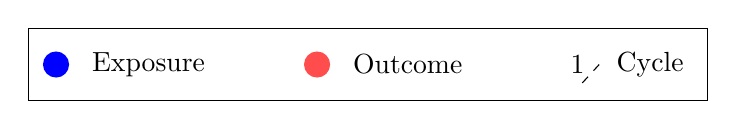
\begin{tikzpicture}
\node (E)[outer sep=2pt,fill = blue, circle] {};
\node (Exposure)[right = 1pt of {E}, outer sep=2pt,fill = white] {Exposure};
\node (O)[right = of {Exposure}, outer sep=2pt,fill = red!70, circle] {};
\node (Outcome)[right = 1pt of {O}, outer sep=2pt,fill = white] {Outcome};
\node (C)[right = of {Outcome}, outer sep=2pt,fill = white] {1};
\path [draw, dashed] (C.east) -- (C.south);
\node (Cycle)[right = 1pt of {C}, outer sep=2pt,fill = white, rectangle] {Cycle};
\node (box1) [draw,solid,fit = (E)(Cycle), outer sep = 6pt]{};
\end{tikzpicture}
\end{center}
\caption{Data availability for exposure and outcome depends on year of birth (which determines age at entry to the cohort). Diagonal dashed lines indicate cycles of the survey. Blue represents time when play can be measured. Orange represents time when health risk behaviours can be measured. Measurement occurs at the intersection of the dashed lines and the coloured lines.}
\end{figure}
\newpage
\subsubsection{Missing Data}

Three separate mechanisms for missing data exist in this dataset. 
\paragraph{Systematic Missing Data by Birth Year.} As shown in Figure 7, there is a systematic lack of data on exposure for children with earlier birth years and a lack of some outcome data for children with later birth years because of how the survey was conducted. A sensitivity analysis could be conducted by restricting the sample to children born between 1987 and 1992.
\paragraph{Loss to Followup.} Over the course of the study, approximately one third of the participants were lost to followup. If the participants who drop out of the study have a different association between health risk behaviour and outdoor active play than those who remain, estimates of effect could suffer from a selection bias. Comparisons of baseline characteristics of these two groups could give an initial idea of the extent of this bias. 
\paragraph{Question Non-Response.} As with any survey, some individual questions will not be answered by participants. Multiple Imputation can be used to recover these observations as long as the data are missing at random (conditional on observed covariates). Questions on health risk behaviour could be missing not at random (MNAR) if participants who (for example) have tried smoking differentially refuse to answer the question. 
\noindent

%\subsubsection{Correlated Effects of Outdoor Active Play at Different Ages}

%The model of the effect of outdoor active play on behaviour should ensure that the effect should be similar for similar ages. This likely means that a multilevel model will be required to pool adjacent estimates. Random walk priors could be used to constrain estimates to be similar for similar ages.~\cite{Ghitza2014-rs} The effect should also generally decrease as age increases, as younger children have higher neuroplasticity (behaviour can cause more significant changes to their brains).~\cite{Mundkur2005-ws} This decrease may not be linear. 

\subsubsection{Assumptions for Causal Inference}

In order to estimate the causal effect of childhood outdoor active play on adolescent health risk behavior, we need some conditions to be true.~\cite{Hernan_undated-yr} The assumptions and some comments on their plausibility follow: 

\paragraph{Exchangeability} requires that children with low outdoor active play and high outdoor active play are otherwise exchangeable (conditional on some set of confounders L). This condition means that - for all two-group sets of children with identical levels of all variables L -  switching their mean exposure would switch their mean outcome. Unmeasured confounding and selection bias are threats to exchangeability. In this study, there are some possible confounders for which we do not have a measure: childhood maltreatment and residential mobility. Analysis without these covariates will require that we assume they have a small effect on exposure or outcome, that the are very uncommon, or that they do not enable an unblocked backdoor path from exposure to outcome. 

\paragraph{Positivity} requires that the distribution of covariates L in children with low outdoor active play completely overlaps the distribution of L in children with high outdoor active play. Testing of this assumption can be accomplished via parametric bootstrapping and deviations can be addressed by reducing the number of parameters in the model, redefining parameters in the model, or restriction of the sample.~\cite{Petersen2010-co}

\paragraph{Well Defined Intervention.} The numerical value of the effect estimate depends on what are considered to be the intervention and control conditions. This is especially important in longitudinal data. The proposed causal effects of interest are the total effect of play at specific time points. Total effects include the direct effect of the exposure at the time point in question as well as the effect that that exposure has though future exposures which are caused by it; in this case, if play at time 1 has an effect on play at time 2, then some portion of the effect of play at time 2 on health risk behaviours should be attributed to play at time 1. This formulation allows estimation of the overall effect of a hypothetical intervention which increased play at any given time point.

\paragraph{Measurement Error and Model Misspecification.} Measurement error in the treatment, outcome, or confounders can result in bias in the causal effect estimate. The most likely source of measurement error in this study is on the exposure, which is measured once for each two year period and then extrapolated to the remaining weeks. Measurement of the confounding variables will be imperfect as well. Multiple models will be fit and compared, but perfect model fit can never be guaranteed. 


\begin{figure}
\centering
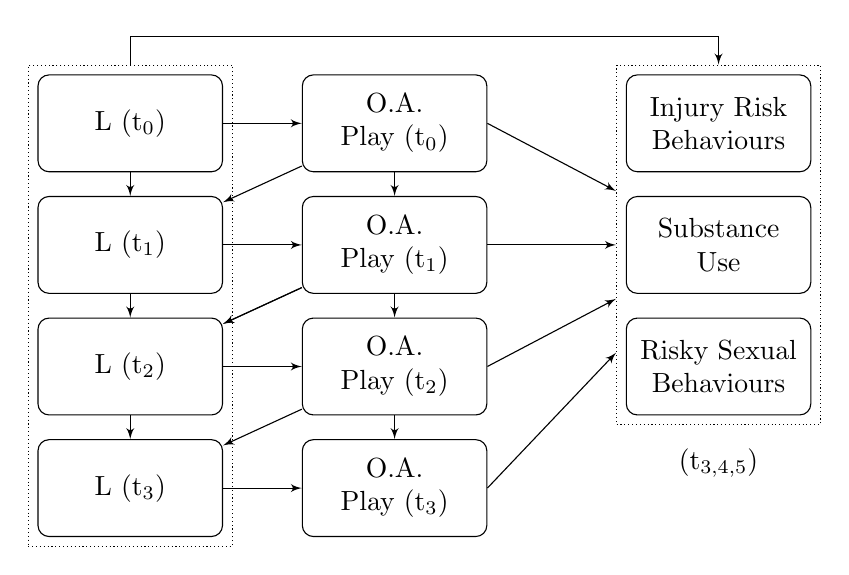
\begin{tikzpicture}[decision/.style={diamond, draw, text width=4.5em,text badly centered, node distance=3.5cm, inner sep=0pt},block/.style={rectangle, draw, text width=6em, text centered,rounded corners, minimum height=3.5em},cloud/.style ={draw, ellipse, minimum height=2em},line/.style ={draw,-latex'},node distance =1cm,auto]
\node [block] (1st) {L (t\textsubscript{1})};
\node [block, right= of 1st] (2nd1) {O.A. Play (t\textsubscript{1})};

\begin{scope}[node distance=3mm and 10mm]
\node [block, above= of 2nd1] (2nd2) {O.A. Play (t\textsubscript{0})};
\node [block, below= of 2nd1] (2nd3) {O.A. Play (t\textsubscript{2})};
\node [block, right= 50pt of 2nd1] (3rd1) {Substance Use};
\node [block, below = of 3rd1] (3rd0) {Risky Sexual Behaviours};
\node [block, above = of 3rd1] (3rd2) {Injury Risk Behaviours};
\node [block, below = of 2nd3] (2nd4) {O.A. Play (t\textsubscript{3})};
\node [block, below = of 1st] (1st2) {L (t\textsubscript{2})};
\node [block, below = of 1st2] (1st3) {L (t\textsubscript{3})};
\node [block, above = of 1st] (1st0) {L (t\textsubscript{0})};
\end{scope}

\draw[line] (2nd2) -- (2nd1);
\draw[line] (2nd1) -- (2nd3);
\draw[line] (2nd3) -- (2nd4);
\draw[line] (1st0) -- (2nd2);
\draw[line] (2nd2) -- (1st);
\draw[line] (1st) -- (2nd1);
\draw[line] (2nd1) -- (1st2);
\draw[line] (2nd1) -- (1st2);
\draw[line] (1st2) -- (2nd3);
\draw[line] (2nd3) -- (1st3);
\draw[line] (1st0) -- (1st);
\draw[line] (1st) -- (1st2);
\draw[line] (1st2) -- (1st3);
\draw[line] (1st3) -- (2nd4);


\node[draw,densely dotted,fit=(3rd0) (3rd2)] (box1){};
\node[draw,densely dotted,fit=(1st0) (1st3)] (box2){};
\node[above = 10pt of 2nd2] (c1) {};

\node[below = 5pt of box1]{(t\textsubscript{3,4,5})};

\draw[line] (2nd1.east) -- (box1);
\draw[line] (2nd4.east) -- (box1);
\draw[line] (2nd2.east) -- (box1);
\draw[line] (2nd3.east) -- (box1);

\draw[draw] (box2) |- (c1.east);
\draw[line] (c1.east) -| (box1);

\end{tikzpicture}
\caption{Relationship of play and the set of confounders (L) from t\textsubscript{0} (Age 6) to outcome assessment (t\textsubscript{3,4,5}). Individual's confounder set L changes over time as a result of both play and external factors. This confounder set influences both future play and eventual outcome.}
\label{timefig}
\end{figure}

\subsubsection{Time-Varying Confounders}

Ethnicity and sex are constant, but all other variables are potentially time-varying. Changes in these variables could be related to outdoor active play activity, either as a cause or an effect (See Figure 8). Models will incorporate changes in these covariates over time if necessary. 

\subsubsection{Sampling Variance}

The NLSCY includes a standard set of bootstrap weights for use in calculating variance inflation due to the survey design. Procedures outlined in the NLSCY microdata user's guide will be followed \cite{noauthor_undated-nd}. 

\subsubsection{Power and Sample Size}

Simulations indicate that with 10,268 sets of 4 observations and a continuous outcome, 80\% power would be reached if the difference between a overall high play and overall low play was greater than 0.33 standard deviations on the outcome scale (assuming equal standard deviation in both groups). 


\section{Potential Covariates.} Confounding variables will be selected based on past literature support of association with exposure or outcome and availability in the dataset. A preliminary list of variables that may be associated with outdoor active play and/or health risk behaviours follows:

\subsection{Effect Modifiers} 

\paragraph{Sex.} Sex will be considered as an effect modifier because boys and girls have both different play experiences and different motivations for health risk behaviour.~\cite{Schuster2013-rz}  Boys and girls also interact with their environment in different ways.~\cite{Bocarro2015-mk, Kaczynski2013-hz, Haug2010-he, Pawlowski2016-vx} Boys spend more time in general in outdoor active play \cite{Bringolf-Isler2010-ma,Lee2016-rb} and are more prone to health risk behaviors than girls.~\cite{Simmons2016-vg,Wellman2016-yp} Boys are significantly more likely to engage in multiple risk behaviors than girls.~\cite{Filippidis2016-qo}

\paragraph{Age.} Increasing age is linked to decreasing outdoor active play and physical activity \cite{Bringolf-Isler2010-ma,Uijtdewilligen2011-km}. The long term behavioural effect of outdoor active play is also expected to fall off as children age as younger children have higher neuroplasticity.~\cite{Chambers2003-db} Younger people are more likely to display multiple risk behaviors,\cite{Filippidis2016-qo} but substance use is more common in older adolescents.~\cite{Wellman2016-yp}

\subsection{Measured Confounders}

\paragraph{Physical Health.} Physical disabilities are associated with reduced outdoor active play \cite{Kolehmainen2015-xn} Chronic pain disorders associated with substance use.~\cite{McLaren2017-gl} Children with physical health issues interact with their environment differently.~\cite{An2017-my,Moore2015-gr,Crawford2014-sy}  The effect of ethnicity, income, education on substance use depends on disability status in adults.~\cite{Courtney-Long2017-bz}

\paragraph{Rurality.} Rurality is associated with an increase in outdoor active play of .28 hours/day.  \cite{Lee2016-rb} Rural adolescents have a 25.8\% higher rate of binge drinking than urban adolescents and may initiate substance use earlier.~\cite{noauthor_undated-so} There are also small but non-significant differences in the rates of other substance use. Decision making around substance use in rural males depends on group membership and perceptions of health risks - with users and non-users disagreeing on the immediacy, severity, and inevitability of the health risks of use.~\cite{Couch2017-tb} The suitability of neighborhoods for play varies between urban and rural neighborhoods; for example, traffic speeds tend to be higher in rural neighbourhoods.~\cite{McAndrews2016-kk}

\paragraph{Ethnicity.} Ethnicity influences attitudes toward violence \cite{Galano2017-yv} and is associated with physical inactivity and sedentary behaviour\cite{Uijtdewilligen2011-km,Salmon2011-co} and substance use, with odds ratios vs. Caucasian rangin from 0.55 - 1.58 for binge drinking and from 0.73 to 1.63 for smoking.~\cite{Shih2010-yv} It is also correlated with outdoor active play behaviours. Amounts of time spent in outdoor active play vary by approximately 0.5 hours per day between the highest and lowest groups.~\cite{Lee2016-rb} Access to neighbourhood play spaces varies by ethnicity in the United States, with hispanic children having the most and white children having the least~\cite{Bottino2012-ja}, but it is unclear whether this pattern would generalize to a Canadian context. 

\paragraph{Socioeconomic Status.} Children from medium socioeconomic status households engage in more outdoor active play than those from low or high socioeconomic status households (+15.6 min/day (0.3, 30.9))\cite{Bringolf-Isler2010-ma}. Lower socioeconomic status is linked to alcohol use (OR 2.63(1.39, 4.95))\cite{Patrick2012-ed}, smoking \cite{Wellman2016-yp}, marijuana use (OR 2.16 (1.32, 3.53))\cite{Patrick2012-ed}, and multiple risk behavior (2.63 (2.12, 3.26))\cite{Filippidis2016-qo}. Attempts to quantify the quality of outdoor active play spaces in low and high SES neighborhoods show dramatic differences on almost all measures of quality.~\cite{Jenkins2015-ru} However, areas of with low SES don't have significant differences in parental perception of risk.~\cite{Moussa2013-dw}

\paragraph{Sleep.} Short sleepers have reduced hours of outdoor active play.~\cite{Kjeldsen2014-kc} Insufficient sleep is also associated with increased smoking, alcohol use, and drug use in rural adolescents in the US.~\cite{Reichenberger2016-cg} The physical environment impacts sleep through traffic noise (High traffic is associated with a decrease of 19.2 min/night of sleep vs. low traffic) or through excessive light at night.~\cite{Bottino2012-ja} 

\paragraph{Family.} Children in single-parent households play 9.9 min/day (2.2, 22.4) more than children in multi-parent households.~\cite{Bringolf-Isler2010-ma} Number of siblings is not associated with increased outdoor active play time.~\cite{Arcury2017-jd} Higher maternal stress is associated with reduced outdoor active play.~\cite{OConnor2017-fq} Adolescents in secure parent-adolescent dyads are less likely to engage in risky sexual behaviours and substance misuse.~\cite{Kobak2017-ia} Parallel process latent growth models indicate parenting style influences externalizing behavior including violence and substance misuse \cite{Wiggins2015-on}. Having brothers can increase the likelihood of substance use.~\cite{Samek2015-sm} Adolescents with low family attachment have higher substance use and higher rates of risky sexual behavior.~\cite{Cordova2016-rb,Samek2015-sm} High parental involvement reduces rates of substance use.~\cite{Samek2015-sm} Parents' perception of neighborhood safety increases outdoor active play time.~\cite{Xu2017-ar}

\paragraph{Mental Health.} Poor mental health is known to reduce childhood physical activity and could reduce outdoor active play as well.~\cite{Boone2016-np} Poor mental health is associated with increases in risky sexual behaviour and substance use.~\cite{McLaren2017-gl} Poor mental health could be influenced by the built environment.~\cite{Min2017-di,Reklaitiene2014-vj}

\subsection{Unmeasured Confounders}

\paragraph{Residential Mobility.} Children whose parents move more often are more likely to engage in overt risk behaviours.~\cite{Brown2012-sc} However, most of this association is due to underlying differences between children who move often and those who do not.~\cite{Morris2016-gu} Residential mobility is also associated with poor neighbourhood quality.~\cite{Kearns2015-nd}

\paragraph{Childhood Maltreatment.} Victims of child maltreatment engage in less outdoor active play.~\cite{Darwish2001-ti,Howard1986-uu} Childhood maltreatment (physical, sexual, and neglect) is linked to risky sexual behavior in female adolescents, an effect mediated by substance use and psychological distress.~\cite{Clements-Nolle2017-ox} Abuse is also linked to behaviors that indicate poor risk assessment such as increased gambling behavior.~\cite{Lane2016-bw} Some evidence suggests that the rate of child abuse varies based on neighbourhood environment.~\cite{Freisthler2008-pp}

\begin{table}[h]
\centering
\begin{tabular}{ m{4cm} p{4cm} p{4cm} p {4cm}}
\toprule
& Outdoor Active Play & Health Risk Behaviour & Built Environment \\
\midrule
Male Sex & + & ++ & N/A \\
Increased Age & --  -- & ++ & N/A \\
SES & -- & ++ & ++ \\
Mental Health & -- -- & -- & -- -- \\
Physical Health & -- & -- -- & -- \\
Residential Mobility & U & ++ & -- \\
Ethnicity & Mix & Mix & Mix \\
Sleep & + & -- -- & -- \\
Abuse & -- & ++ & + \\
Rurality & + & ++ & + \\
Family Structure & -- & Mix & U \\
Family Attachment & U & --  -- & U \\
Family Environment & + & -- & U \\
\bottomrule
\multicolumn{4}{p{17cm}}{U = unknown, -- -- = strong evidence for negative association, -- = weak evidence for negative association, + weak evidence for positive association, ++ = strong evidence for positive association, Mix = mixed evidence.}\\ 
\end{tabular}
\caption{Known associations between outdoor active play, health risk behaviour, built environment, and covariates.}
\end{table}

\section{Additional Considerations}

\subsection{Overall Strengths and Limitations}

This proposed thesis project proposes to examine the causal links from environment through outdoor active play to health risk behaviors. By accessing three different Canadian data sources, we hope to provide a balanced picture of this causal pathway. However, there are some limitations to what can be accomplished. The most recent longitudinal data source is more than 10 years old, and children may have different experiences now than they did in the past due in part to the increase in time spent online over this time period. Evaluation of the causal effects of neighbourhood-level exposures from observational data is difficult due to potential for bias due to self-selection into neighbourhoods. Lack of data on the amount of time spent in each activity necessitates assumptions in order to compare injury risks. The cross sectional nature of the data for manuscripts one and two also force certain assumptions. For manuscript one, we need to assume that the current state of the neighbourhood as observed represents the neighbourhood in the recent past when it was influencing outdoor active play. For manuscript two, we need to assume that previous injuries do not change the probability of injury for individuals. 

\subsection{Ethical considerations:} This proposed project will undergo ethics review by the Queen's University HSREB.  

\paragraph{Informed Consent:} \emph{HBSC.} Informed consent is sought from both pupils and their parents or guardians (explicit or implicit, based on local school board custom), as participants are under the age of consent.~\cite{noauthor_undated-do} \emph{NLSCY.} Explicit informed consent was obtained from the parent or legal guardian of all children enrolled in the study. \emph{CHIRPP.} Consent is obtained from patients prior to data collection. 
\paragraph{Harm Reduction:} Care will be taken to prevent any individually identifiable data from being released. Data safety for the HBSC will be ensured by holding data on a password protected computer on site at Carruthers Hall, Queen's University. All work with data from the NLSCY will be completed at the Queen's Research Data Centre. CHIRPP data will be held onsite at KGH on a hospital network computer. 

\paragraph{Outputs:} In order to ensure benefits are realized from this project, appropriate knowledge translation projects, including open access publications, infographics, interactive visualizations,\cite{noauthor_undated-gc} and/or guidelines for neighbourhood planning will be developed. If possible, a tool for calculating the playability index will be developed that can be used by any interested party. The specific nature of these projects and their target audience will depend on the findings.  

\subsection{Appropriateness for a PhD in Epidemiology.} 

\paragraph{Project Suitability.} This project involves three different epidemiological study designs (one descriptive, one cross-sectional, one longitudinal), each with their own set of challenges. With respect to other methodological requirements, development of the classification algorithm for manuscript two, collection of neighbourhood features using GIS in manuscript one, and linking and managing the cycles of the NLSCY all represent significant time commitments. Data collection in the form of environmental data to inform the playability measure used in manuscript one and chart reviews for manuscript two will be completed by the student. Manuscripts one and three involve complex modelling challenges. In all manuscripts, care will be taken to use current epidemiological principles to maximize internal validity. The project scope has been approved at the outline stage of review. 

\paragraph{Contributions of the Student.} The project as proposed is to be completed primarily by the student with support from the supervisory team: Drs. William Pickett and Ian Janssen. Ideas for the manuscripts were developed by the State of Play team at UBC, by Drs. Pickett and Janssen, and by the student. 

\paragraph{Feasibility:} Access to the HBSC data will be facilitated by Drs. Pickett and Janssen, two of the Canadian HBSC investigators. Access to the NLSCY data will require a project proposal to be submitted to and approved by SSHRC; other Ph.D. students of Drs. Pickett and Janssen have previously gone through this process. Access to Kingston CHIRPP data will be obtained with help from Dr. Rob Brison and Dr. Chris Evans, colleagues of Dr. Pickett's. I have applied for funding to attend a workshop in Causal Inference from Observational data. 


\begin{table}[h]
\begin{center}
\begin{tabular}{ m{6cm} m{6cm} }
\toprule
Item & Timeframe \\
\midrule
Proposal Presentation & Fall 2018 \\
Manuscript Preparation & Fall 2018 - Winter 2019 \\ 
Writing Thesis & January 2020 - Summer 2020 \\
Thesis Defence & August 2020 \\
\bottomrule
\end{tabular}
\caption{Timeline of project completion.}
\end{center}
\end{table}

\newpage
\bibliography{prop31}{}
\bibliographystyle{unsrt}

\newpage
\section{Appendix A: Comments on Suggested Improvements}

\subsection*{Outline Feedback}

\paragraph{Comment 1.}Suitability as a PhD in Epidemiology.  The committee agreed that the project as proposed: (1) would be suitable in terms of the amount of work (if anything, too ambitious; (2) was cohesive and fit together thematically; (3) involved multiple datasets with different challenges and opportunities; (4) had depth of statistical and methodological complexity consistent with what was required in our department.

\paragraph{Response 1.} Changes have been made to the scope - reduced number of years in the CHIRPP study and focused the definition of risk behavior.

\paragraph{Comment 2.}Conceptual Framework.  There is a need for a more comprehensive conceptual framework that builds on the existing figure, and considers risk behaviours, healthy behaviours, and other covariates, and directs the reader to which of these will be a focus.

\paragraph{Response 2.}Figures have been added to this effect (Figures 1 and 3)
 
\paragraph{Comment 3.}Rates (manuscript 1 [now 2]).  There needs to be a clear and informed section of the proposal that addresses how the denominators will be created for the Kingston area hospitals, so that rates can be calculated.

\paragraph{Response 3.}This section has been added (Section REF)

\paragraph{Comment 4.}Scope (manuscripts 1,3).  There were concerns expressed around the scope of the manuscripts, and specifically: (a) Manuscript 1;  20 years of data; 4 types of activity leading to injury; many covariates; and the recommendation was to make some practical decisions so that the scope for the data collection, analysis and its interpretation could be done in one paper;  (b) Manuscript 3;  the scope and practicality of measuring the playability index for all participants was questioned.  It was recommended that we need to consider the feasibility of having the measured required for the playability index via an automated process, and have multiple options considered in the proposal should the preferred option not be feasible.  (c) there was concern that Randy examines the scope of the entire project, and be prepared to make some decisions to cut if it is not feasible to complete within the remaining PHD time (2 and a bit years).

\paragraph{Response 4.}See point 1.

\paragraph{Comment 5.}Functional Logistic Regression.  Recommendation is that the statistical approach used for the longitudinal analysis may not be optimal, and Randy should examine other options (e.g., logistic or another regression method, with conventional approaches to time-dependent covariate data).  Need to also consider the timing of the measures and developmental stages of children in making these decisions.

\paragraph{Response 5.}The suggestion of functional logistic regression has been removed. A discussion of the particular demands of this project and expected obstacles has been added.

\paragraph{Comment 6.}Ensure that writing is polished, and tells a cohesive and progressive story, and that the objectives and hypotheses are explicit.

\end{document}

